\documentclass[xcolor=svgnames, 8pt, handout, standalone]{beamer}
\input{beamerUVApreamble}
\usepackage{microtype}
\usepackage{multicol}
\usepackage{bm}
\usepackage{etoolbox}
\usepackage{tcolorbox}
\tcbuselibrary{skins}
\usepackage{listings}
\usetikzlibrary{matrix}
\lstset{
    basicstyle=\ttfamily\footnotesize,
    keywordstyle=\color{blue},
    commentstyle=\color{green},
    breaklines=true
}

% SHORTCUTS
\newcommand{\Var}{\operatorname{Var}}
\newcommand{\Cov}{\operatorname{Cov}}
\newcommand{\1}{\mathbf{1}}
\newcommand{\R}{\mathbb{R}}
\newcommand{\KL}{\mathrm{D}_{\mathrm{KL}}}
\newcommand{\I}{\mathbf{I}}
\newcommand{\softmax}{\operatorname{softmax}}
\newcommand{\sigmoid}{\operatorname{sigmoid}}
\newcommand{\principle}[1]{\textbf{#1}}
\newcommand{\reasonprompt}[1]{\par\small\emph{Reasoning prompt:} #1}
\definecolor{deepblue}{RGB}{0,51,102}
\definecolor{deepgreen}{RGB}{0,102,51}
\definecolor{deepred}{RGB}{153,0,0}
\definecolor{lightblue}{RGB}{230,240,250}
\definecolor{lightyellow}{RGB}{255,250,230}
\definecolor{vibrantblue}{RGB}{0,123,255}
\definecolor{energyorange}{RGB}{255,149,0} 
\definecolor{hotpink}{RGB}{255,45,85}
\definecolor{electricpurple}{RGB}{147,51,234}
\definecolor{neongreen}{RGB}{57,255,20}

\title{From Classification to Optimization}
\subtitle{Loss Functions and Stochastic Gradient Descent}
\author{Heman Shakeri}
\date{}

\begin{document}

\begin{frame}
\titlepage
\end{frame}

\begin{frame}{Recap: From Regression to Classification}
\textbf{In the previous videos we covered:}
\begin{itemize}
\item Linear regression
\item MSE loss: $\mathcal{L} = \frac{1}{n}\sum_i (y_i - \hat{y}_i)^2$
\item Nice properties:
    \begin{itemize}
    \item Convex
    \item Simple gradient
    \end{itemize}
\end{itemize}
\begin{tcolorbox}[colback=lightyellow, colframe=energyorange, boxrule=1pt]
\centering
\textbf{Next Question:} How do we adapt our loss functions for classification?
\end{tcolorbox}
\end{frame}


% Add this NEW SECTION after the "Recap: From Regression to Classification" frame
% and BEFORE the "Binary Classification: The Setup" frame

\begin{frame}{Classification and Regression: More Similar Than You Think!}
\begin{columns}
\begin{column}{0.48\textwidth}
\begin{block}{Regression}
\textbf{Goal:} Predict continuous value
\begin{equation*}
y \in \mathbb{R}
\end{equation*}
\textbf{Output:} Direct prediction
\begin{equation*}
\hat{y} = f(x; \theta)
\end{equation*}
\textbf{Loss:} Mean Squared Error
\begin{equation*}
\mathcal{L} = \frac{1}{2}(\hat{y} - y)^2
\end{equation*}
\end{block}
\end{column}
\begin{column}{0.48\textwidth}
\begin{block}{Classification}
\textbf{Goal:} Predict category
\begin{equation*}
y \in \{0, 1, \ldots, C-1\}
\end{equation*}
\textbf{Output:} Probabilities
\begin{equation*}
\hat{p} = \sigma(f(x; \theta))
\end{equation*}
\textbf{Loss:} Cross-Entropy
\begin{equation*}
\mathcal{L} = -y\log(\hat{p})
\end{equation*}
\end{block}
\end{column}
\end{columns}

\vspace{0.5cm}
\pause
\begin{tcolorbox}[colback=lightyellow, colframe=hotpink, boxrule=2pt]
\centering
\textbf{But in practice, they're more similar than different!}
\end{tcolorbox}
\end{frame}

\begin{frame}{The Modern View: Logits Unify Everything}
\begin{block}{What Actually Happens in Classification}
The network doesn't directly predict probabilities. Instead:
\begin{enumerate}
\item Network produces \textbf{logits} (unconstrained real numbers): $o = f(x; \theta)$
\item Logits go through activation: $\hat{p} = \sigma(o)$ or $\softmax(o)$
\item Loss computed on probabilities: $\mathcal{L} = -\sum y \log(\hat{p})$
\end{enumerate}
\end{block}

\pause
\begin{tcolorbox}[colback=lightblue, colframe=deepblue, boxrule=2pt]
\textbf{Key:} Predicting logits $o \in \mathbb{R}$ is \textbf{regression}!\\
Classification = Regression (logits) + Activation + Different Loss
\end{tcolorbox}
\end{frame}

\begin{frame}{Side-by-Side: The Parallel Structure}
\begin{center}
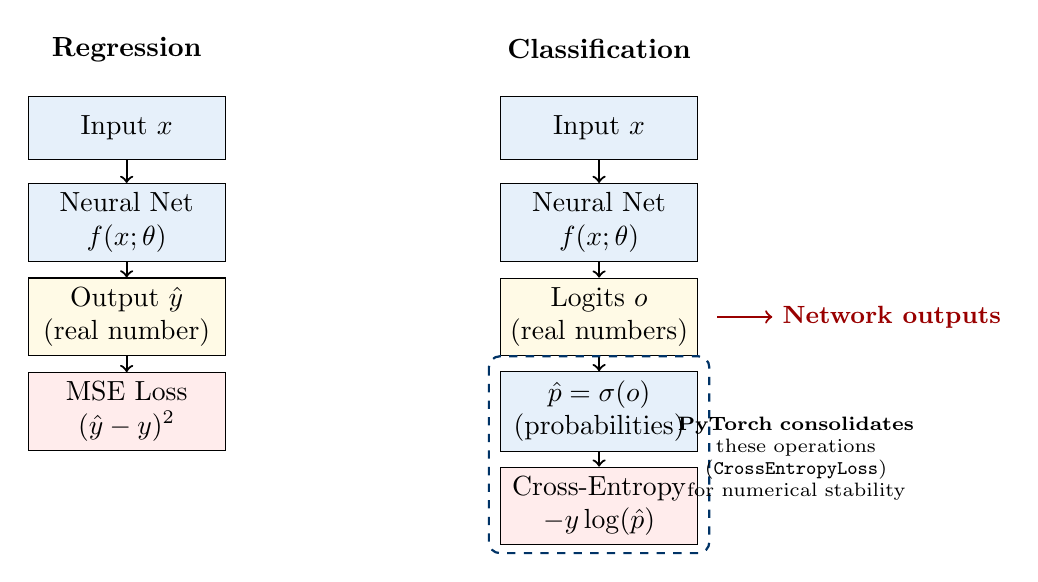
\begin{tikzpicture}[
    block/.style={rectangle, draw, minimum width=2.5cm, minimum height=0.8cm, align=center, fill=lightblue},
    arrow/.style={->, thick}
]
    % Regression path
    \node at (-3, 4) {\textbf{Regression}};
    \node[block] (reg_input) at (-3, 3) {Input $x$};
    \node[block] (reg_net) at (-3, 1.8) {Neural Net\\$f(x; \theta)$};
    \node[block, fill=lightyellow] (reg_out) at (-3, 0.6) {Output $\hat{y}$\\(real number)};
    \node[block, fill=pink!30] (reg_loss) at (-3, -0.6) {MSE Loss\\$(\hat{y} - y)^2$};
    
    \draw[arrow] (reg_input) -- (reg_net);
    \draw[arrow] (reg_net) -- (reg_out);
    \draw[arrow] (reg_out) -- (reg_loss);
    
    % Classification path
    \node at (3, 4) {\textbf{Classification}};
    \node[block] (cls_input) at (3, 3) {Input $x$};
    \node[block] (cls_net) at (3, 1.8) {Neural Net\\$f(x; \theta)$};
    \node[block, fill=lightyellow] (cls_logit) at (3, 0.6) {Logits $o$\\(real numbers)};
    \node[block, fill=lightblue] (cls_prob) at (3, -0.6) {$\hat{p} = \sigma(o)$\\(probabilities)};
    \node[block, fill=pink!30] (cls_loss) at (3, -1.8) {Cross-Entropy\\$-y\log(\hat{p})$};
    
    \draw[arrow] (cls_input) -- (cls_net);
    \draw[arrow] (cls_net) -- (cls_logit);
    \draw[arrow] (cls_logit) -- (cls_prob);
    \draw[arrow] (cls_prob) -- (cls_loss);
    
    % Dashed box around softmax + cross-entropy
    \draw[dashed, thick, deepblue, rounded corners] 
        (1.6, 0.1) rectangle (4.4, -2.4);
    
    % Label for the dashed box
    \node[align=center, text width=3.2cm, font=\scriptsize] at (5.5, -1.2) {
        \textbf{PyTorch consolidates}\\
        these operations\\
        (\texttt{CrossEntropyLoss})\\
        for numerical stability
    };
    
    % Annotation for network output
    \draw[->, deepred, thick] (4.5, 0.6) -- (5.2, 0.6) 
        node[right, font=\small\bfseries, text=deepred] {Network outputs};
\end{tikzpicture}
\end{center}

\pause
\vspace{0.3cm}
\textbf{Notice:} Both predict \textcolor{orange}{unconstrained real values (logits)}!
\end{frame}

\begin{frame}{Why Logits? Three Compelling Reasons}
\begin{enumerate}
\item<1-> \textbf{Numerical Stability}
\begin{itemize}
\item Probabilities near 0 or 1 cause $\log(0)$ disasters
\item Logits stay in safe numerical range
\item Combined softmax + cross-entropy is stable
\end{itemize}

\vspace{0.3em}
\item<2-> \textbf{Separation of Concerns}
\begin{itemize}
\item Network learns \textit{unconstrained} representations (logits)
\item Activation handles probability constraints
\item Cleaner optimization landscape
\end{itemize}

\vspace{0.3em}
\item<3-> \textbf{Gradient Beauty}
\begin{itemize}
\item Remarkable simplification (we'll see this shortly!)
\item Activation derivative cancels with loss derivative
\item Simple "error signal" for learning
\end{itemize}
\end{enumerate}
\end{frame}

\begin{frame}{Unified Network Design: One Architecture, Many Tasks}
\begin{center}
\begin{tikzpicture}[scale=0.9, transform shape]
    \node[draw, rectangle, minimum width=3.5cm, minimum height=1.8cm, fill=lightblue, align = center] (net) at (0,0) {
        \textbf{Shared Neural Network}\\
        (feature learning)\\
        layers 1 to $L-1$
    };
    
    \node[draw, rectangle, fill=lightyellow, minimum width=2.5cm, align = center] (reg_head) at (-3, -2.8) {
        \textbf{Regression Head}\\
        Linear output\\
        $\hat{y} = Wo + b$
    };
    \node[draw, rectangle, fill=lightyellow, minimum width=2.5cm, align = center] (cls_head) at (3, -2.8) {
        \textbf{Classification Head}\\
        Softmax\\
        $\hat{p} = \softmax(o)$
    };
    
    \draw[->, thick, deepblue] (net) -- (reg_head);
    \draw[->, thick, deepred] (net) -- (cls_head);
    
    \node[below=0.2cm of reg_head, font=\small] {MSE Loss};
    \node[below=0.2cm of cls_head, font=\small] {Cross-Entropy Loss};
\end{tikzpicture}
\end{center}

\pause
\vspace{0.5em}
\begin{columns}
\begin{column}{0.48\textwidth}
\textbf{What changes:}
\begin{itemize}
\item Final activation (identity vs softmax)
\item Loss function (MSE vs CE)
\end{itemize}
\end{column}
\begin{column}{0.48\textwidth}
\textbf{What stays the same:}
\begin{itemize}
\item Network architecture
\item Feature learning principles
\item Optimization (SGD, Adam)
\end{itemize}
\end{column}
\end{columns}
\end{frame}

\begin{frame}{Practical Implications for Network Design}
\begin{tcolorbox}[colback=lightyellow, colframe=energyorange, boxrule=2pt]
\centering
\textbf{Modern Deep Learning Philosophy:}\\
95\% shared representation learning + 5\% task-specific head
\end{tcolorbox}

\vspace{0.5em}
\textbf{Design Strategy:}
\begin{enumerate}
\item \textbf{Layers 1 to $L-1$:} Representation Learning
\begin{itemize}
\item Extract useful features from input
\item Build hierarchical abstractions
\item \textcolor{deepblue}{Same for regression and classification!}
\end{itemize}

\vspace{0.3em}
\item \textbf{Final Layer + Loss:} Task-Specific Head
\begin{itemize}
\item Regression: Linear layer + MSE
\item Binary Classification: Sigmoid + BCE
\item Multi-class: Softmax + Cross-Entropy
\item Multi-label: Multiple sigmoids + BCE per class
\end{itemize}
\end{enumerate}

\pause
\vspace{0.3em}
\begin{tcolorbox}[colback=lightblue, colframe=deepblue, boxrule=1pt]
\textbf{Key Takeaway:} Don't think "regression vs classification"\\
Think: \textbf{representation learning + appropriate output head}
\end{tcolorbox}
\end{frame}

\begin{frame}{Binary Classification: The Setup}
\begin{columns}
\begin{column}{0.5\textwidth}
\textbf{The Problem:}
\begin{itemize}
\item Predict discrete classes: $y \in \{0, 1\}$
\item Examples:
    \begin{itemize}
    \item Email: spam or not spam
    \item Medical: tumor present/absent
    \item Review: positive/negative
    \end{itemize}
\end{itemize}
\vspace{1em}
\textbf{The Challenge:}\\
Model outputs raw scores (logits) $o \in \mathbb{R}$\\
Need probabilities $p \in [0,1]$
\end{column}
\begin{column}{0.5\textwidth}
\begin{center}
\includegraphics[width=0.9\textwidth]{Module 1/Fig5.6.png}\\
{\tiny [Figure from Prince ``Understanding Deep Learning'', Ch. 5]}
\end{center}
\textbf{Bernoulli Distribution:}
$$P(y=1) = \lambda, \quad P(y=0) = 1-\lambda$$
\end{column}
\end{columns}
\end{frame}

\begin{frame}{The Sigmoid Function: From Logits to Probabilities}
\begin{columns}
\begin{column}{0.45\textwidth}
\textbf{Logistic Sigmoid:}
$$\sigmoid(o) = \frac{1}{1 + e^{-o}} = \frac{e^o}{e^o + 1}$$

\textbf{Properties:}
\begin{itemize}
\item Maps $(-\infty, +\infty) \to (0, 1)$
\item Centered: $\sigmoid(0) = 0.5$
\item Smooth and differentiable
\item Saturates at extremes
\end{itemize}
\end{column}
\begin{column}{0.55\textwidth}
\begin{center}
\includegraphics[width=\textwidth]{Module 1/Fig5.7.png}\\
{\tiny [Figure from Prince ``Understanding Deep Learning'', Ch. 5]}
\end{center}
\end{column}
\end{columns}
\vspace{0.5em}
\begin{tcolorbox}[colback=lightblue, colframe=deepblue, boxrule=1pt]
\textbf{Key Insight:} Network outputs logit $o$, sigmoid converts to probability $\hat{p} = \sigmoid(o)$
\end{tcolorbox}
\end{frame}

\begin{frame}{Binary Cross-Entropy Loss}
\begin{block}{The Loss Function}
Given true label $y \in \{0,1\}$ and predicted probability $\hat{p} = \sigmoid(o)$:
$$\mathcal{L}_{\text{BCE}} = -[y \log \hat{p} + (1-y) \log(1-\hat{p})]$$
\end{block}

\begin{columns}
\begin{column}{0.5\textwidth}
\textbf{When $y = 1$:}
$$\mathcal{L} = -\log \hat{p}$$
\begin{itemize}
\item Want $\hat{p} \to 1$
\item Loss $\to 0$ as $\hat{p} \to 1$
\item Loss $\to \infty$ as $\hat{p} \to 0$
\end{itemize}
\end{column}
\begin{column}{0.5\textwidth}
\textbf{When $y = 0$:}
$$\mathcal{L} = -\log(1-\hat{p})$$
\begin{itemize}
\item Want $\hat{p} \to 0$
\item Loss $\to 0$ as $\hat{p} \to 0$
\item Loss $\to \infty$ as $\hat{p} \to 1$
\end{itemize}
\end{column}
\end{columns}
\end{frame}

\begin{frame}{The Beautiful Gradient}
\begin{tcolorbox}[colback=lightyellow, colframe=hotpink, boxrule=2pt]
\centering
\textbf{Magic happens when we combine sigmoid + cross-entropy!}
\end{tcolorbox}

\vspace{1em}
\textbf{Computing the gradient:}
$$\frac{\partial \mathcal{L}}{\partial o} = \frac{\partial \mathcal{L}}{\partial \hat{p}} \cdot \frac{\partial \hat{p}}{\partial o}$$

\vspace{0.5em}
After chain rule and simplification:
$$\boxed{\frac{\partial \mathcal{L}}{\partial o} = \hat{p} - y}$$

\vspace{1em}
\begin{columns}
\begin{column}{0.5\textwidth}
\textbf{This is remarkable!}
\begin{itemize}
\item Same form as MSE gradient
\item Error directly drives update
\item No saturation from sigmoid
\end{itemize}
\end{column}
\begin{column}{0.5\textwidth}
\textbf{Intuition:}
\begin{itemize}
\item If $y=1, \hat{p}=0.9$: small gradient
\item If $y=1, \hat{p}=0.1$: large gradient
\item Gradient $\propto$ prediction error
\end{itemize}
\end{column}
\end{columns}
\end{frame}

\begin{frame}{Multi-Class Classification}
\begin{columns}
\begin{column}{0.5\textwidth}
\textbf{The Setup:}
\begin{itemize}
\item $K$ classes: $y \in \{1, 2, ..., K\}$
\item $K$ logits: $\mathbf{o} = [o_1, ..., o_K]$
\item Need: $K$ probabilities summing to 1
\end{itemize}

\vspace{1em}
\textbf{The Softmax Function:}
$$\softmax_j(\mathbf{o}) = \frac{e^{o_j}}{\sum_{k=1}^K e^{o_k}}$$
\end{column}
\begin{column}{0.5\textwidth}
\begin{center}
\includegraphics[width=0.95\textwidth]{Module 1/Fig5.9.png}\\
{\tiny [Figure from Prince ``Understanding Deep Learning'', Ch. 5]}
\end{center}
\end{column}
\end{columns}

\textbf{Properties:} All outputs positive, sum to one, preserves ordering
\end{frame}

\begin{frame}{Multi-Class Cross-Entropy}
\begin{block}{The Loss Function}
For one-hot encoded label $\mathbf{y}$ and softmax predictions $\hat{\mathbf{y}}$:
$$\mathcal{L}_{\text{CE}} = -\sum_{j=1}^K y_j \log \hat{y}_j = -\log \hat{y}_{\text{true class}}$$
\end{block}

\textbf{The gradient (again beautiful!):} $\frac{\partial \mathcal{L}}{\partial o_j} = \hat{y}_j - y_j$

\begin{center}
\includegraphics[width=1\textwidth]{Module 1/Fig5.10.png}\\
{\tiny [Figure from Prince ``Understanding Deep Learning'', Ch. 5]}
\end{center}

\end{frame}

%% Frame 1: Entropy - The Foundation
\begin{frame}{Entropy: Measuring Uncertainty}

\textbf{What is Entropy?}\\[0.5em]
Entropy quantifies the \textcolor{rred}{average uncertainty} or ``surprise'' in a probability distribution.

\pause
\vspace{0.5em}

\begin{columns}[T]
\begin{column}{0.48\textwidth}
\textbf{Definition:}
$$H(P) = -\sum_{i} p_i \log p_i$$

\pause
\textbf{Intuition:}
\begin{itemize}
    \item High entropy $\rightarrow$ high uncertainty
    \item Low entropy $\rightarrow$ predictable outcomes
    \item $H(P) = 0$ when outcome is certain
\end{itemize}
\end{column}

\pause
\begin{column}{0.48\textwidth}
\textbf{Example: Coin Flip}\\[0.3em]
\begin{tabular}{lcc}
\toprule
\textbf{Coin} & \textbf{$P(\text{heads})$} & \textbf{Entropy} \\
\midrule
Fair & 0.5 & 1 bit \\
Biased & 0.9 & 0.47 bits \\
Two-headed & 1.0 & 0 bits \\
\bottomrule
\end{tabular}
\end{column}
\end{columns}

\pause
\vspace{0.5em}
\begin{block}{Information Theory View}
Entropy $H(P)$ is the \textbf{minimum average bits} needed to encode messages from distribution $P$. It represents the \emph{optimal} compression limit.
\end{block}

\end{frame}

%% Frame 2: From Entropy to Cross-Entropy
\begin{frame}{Cross-Entropy: When Your Model is Wrong}

\textbf{The Problem:} What if we use the \textcolor{rred}{wrong} distribution $Q$ to encode data from the \textcolor{jblue}{true} distribution $P$?

\pause
\vspace{0.5em}

\begin{columns}[T]
\begin{column}{0.48\textwidth}
\textbf{Cross-Entropy:}
$$H(P, Q) = -\sum_{i} p_i \log q_i$$

\pause
\textbf{Interpretation:}
\begin{itemize}
    \item Expected bits using $Q$'s code for $P$'s data
    \item Always $\geq H(P)$ (suboptimal encoding)
    \item Equals $H(P)$ only when $Q = P$
\end{itemize}

\pause
\vspace{0.3em}
\textbf{KL Divergence --- The ``Penalty'':}
$$D_{KL}(P \| Q) = H(P, Q) - H(P)$$
Extra bits wasted by using $Q$ instead of $P$.
\end{column}

\pause
\begin{column}{0.48\textwidth}
\textbf{In Classification:}
\begin{itemize}
    \item $P$: true labels (one-hot)
    \item $Q$: model's predicted probabilities
\end{itemize}

\pause
\vspace{0.3em}
\begin{alertblock}{Key Insight}
For one-hot labels ($p_c = 1$):\\[0.2em]
$H(P) = 0$, so:
$$H(P, Q) = D_{KL}(P \| Q) = -\log q_c$$
This is exactly the cross-entropy loss!
\end{alertblock}

\pause
\vspace{0.3em}
\textbf{Why minimize CE?}\\
Since $H(P)$ is constant:
$$\min H(P,Q) \equiv \min D_{KL}(P \| Q)$$
We push $Q$ toward $P$.
\end{column}
\end{columns}

\end{frame}


\begin{frame}[fragile]{PyTorch's CrossEntropyLoss: The All-in-One Solution}
\begin{tcolorbox}[colback=lightyellow, colframe=energyorange, boxrule=2pt]
\centering
\textbf{Key Insight:} PyTorch's \texttt{CrossEntropyLoss} combines softmax + log + NLL loss internally!
\end{tcolorbox}

\vspace{1em}
\textbf{What happens under the hood:}
\begin{enumerate}
\item Network outputs raw logits: $\mathbf{o} \in \mathbb{R}^K$
\item PyTorch internally computes:
\begin{itemize}
\item Log-softmax: $\log\mathrm{softmax}(\mathbf{o})_j = o_j - \log\sum_{k=1}^K e^{o_k}$
\item Negative log-likelihood for true class $c$: $-\log\mathrm{softmax}(\mathbf{o})_c$
\end{itemize}
\end{enumerate}

\begin{columns}
\begin{column}{0.48\textwidth}
\textbf{$\boldsymbol{\times}$ Don't do this:}
\begin{lstlisting}[language=Python]
# Wrong: applying softmax twice!
output = model(x)  # logits
probs = F.softmax(output, dim=1)
loss = F.cross_entropy(probs, y)
\end{lstlisting}
\end{column}
\begin{column}{0.48\textwidth}
\textbf{$\boldsymbol{\checkmark}$ Correct approach:}
\begin{lstlisting}[language=Python]
# Right: pass logits directly
output = model(x)  # logits
loss = F.cross_entropy(output, y)
# or equivalently:
criterion = nn.CrossEntropyLoss()
loss = criterion(output, y)
\end{lstlisting}
\end{column}
\end{columns}
\end{frame}


\begin{frame}{Label Handling: Why PyTorch Uses Integer Indices}
\textbf{The Question:} How do we represent class labels for the loss function?

\vspace{0.5em}
\begin{columns}
\begin{column}{0.48\textwidth}
\textbf{Traditional: One-Hot Encoding}
\begin{itemize}
\item Class 0 of 5: $[1,0,0,0,0]$
\item Class 2 of 5: $[0,0,1,0,0]$
\item Class 4 of 5: $[0,0,0,0,1]$
\end{itemize}

\vspace{0.3em}
\textbf{Cross-entropy becomes:}
$$\mathcal{L} = -\sum_{j=1}^K y_j \log \hat{y}_j$$

\vspace{0.3em}
Since only one $y_j = 1$, this simplifies to:
$$\mathcal{L} = -\log \hat{y}_c$$
where $c$ is the true class.
\end{column}
\begin{column}{0.48\textwidth}
\textbf{PyTorch: Integer Index}
\begin{itemize}
\item Class 0 of 5: just ``0''
\item Class 2 of 5: just ``2''
\item Class 4 of 5: just ``4''
\end{itemize}

\vspace{0.3em}
\textbf{Loss computation:}
$$\mathcal{L} = -\log \hat{y}_c$$
\textit{where $c$ is the integer label}

\vspace{0.3em}
\textbf{Mathematically identical!}\\
Why store zeros when we only need the index?
\end{column}
\end{columns}
\end{frame}

\begin{frame}{Concrete Example: Batch of 3 Images}
\textbf{Scenario:} Classifying 3 images into 10 classes (e.g., MNIST digits)

\vspace{0.5em}
\begin{columns}
\begin{column}{0.48\textwidth}
\textbf{One-Hot Encoding:}
\begin{itemize}
\item Image 1 is class 3: $[0,0,0,\mathbf{1},0,0,0,0,0,0]$
\item Image 2 is class 7: $[0,0,0,0,0,0,0,\mathbf{1},0,0]$
\item Image 3 is class 1: $[0,\mathbf{1},0,0,0,0,0,0,0,0]$
\end{itemize}

\vspace{0.3em}
\textbf{Storage:}
$$3 \times 10 = 30 \text{ values}$$
(27 zeros, 3 ones)
\end{column}
\begin{column}{0.48\textwidth}
\textbf{Integer Indices:}
\begin{itemize}
\item Image 1 is class 3: \texttt{3}
\item Image 2 is class 7: \texttt{7}
\item Image 3 is class 1: \texttt{1}
\end{itemize}

\vspace{0.3em}
\textbf{Storage:}
$$3 \text{ values}$$

\vspace{0.3em}
\textcolor{deepgreen}{\textbf{10$\times$ memory reduction!}}
\end{column}
\end{columns}

\vspace{0.5em}
\pause
\begin{tcolorbox}[colback=lightyellow, colframe=energyorange, boxrule=1pt]
For 1000 classes: \textbf{1000$\times$ memory savings!}\\
For ImageNet (1.2M images, 1000 classes): Save 4.8GB of memory just for labels!
\end{tcolorbox}
\end{frame}

\begin{frame}[fragile]{How PyTorch Handles Integer Labels Internally}
\textbf{Given:}
\begin{itemize}
\item \texttt{logits}: shape \texttt{[batch\_size, num\_classes]} — raw network outputs
\item \texttt{labels}: shape \texttt{[batch\_size]} — integer class indices
\end{itemize}

\vspace{0.5em}
\textbf{Step-by-step computation:}

\begin{lstlisting}[language=Python]
# Example: batch_size=3, num_classes=5
logits = torch.tensor([[2.0, 1.0, 0.1, 3.0, 0.5],   # sample 0
                       [1.0, 4.0, 2.0, 0.5, 1.5],   # sample 1
                       [0.5, 1.0, 3.5, 2.0, 1.0]])  # sample 2
labels = torch.tensor([3, 1, 2])  # true classes

# Step 1: Compute log probabilities for ALL classes
log_probs = F.log_softmax(logits, dim=1)
# Shape: [3, 5]

# Step 2: Extract ONLY the log prob of the true class for each sample
# This is the magic: use labels to index into log_probs
loss_per_sample = -log_probs[range(3), labels]
# Equivalent to: [-log_probs[0,3], -log_probs[1,1], -log_probs[2,2]]

# Step 3: Average over batch
loss = loss_per_sample.mean()
\end{lstlisting}
\end{frame}

\begin{frame}{The Indexing Magic: Visualized}
\textbf{How PyTorch uses integer labels to extract the right log probability:}

\vspace{1em}
\begin{center}
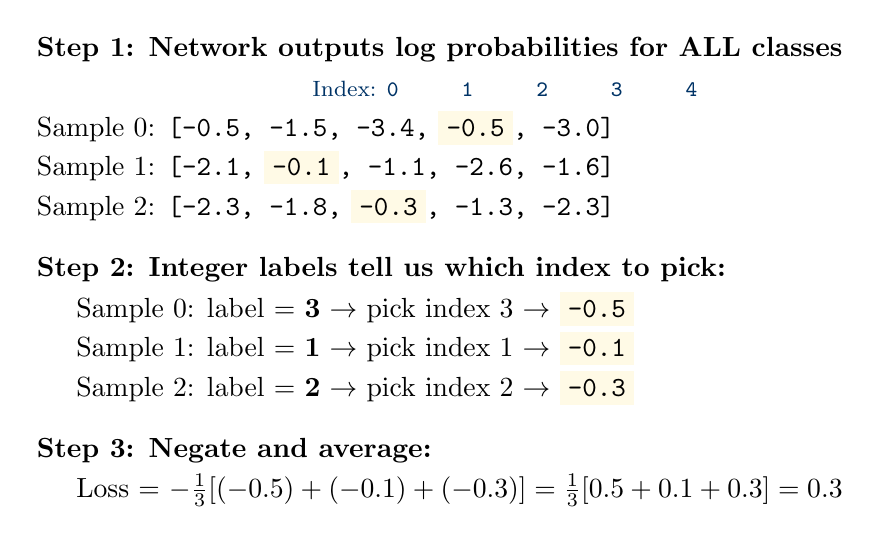
\begin{tikzpicture}[scale=1.0]
    % Title
    \node[anchor=west] at (0, 4) {\textbf{Step 1: Network outputs log probabilities for ALL classes}};
    
    % Log probabilities representation
    \node[anchor=west] at (0, 3) {Sample 0: \texttt{[-0.5, -1.5, -3.4,} \colorbox{lightyellow}{\texttt{-0.5}}\texttt{, -3.0]}};
    \node[anchor=west] at (0, 2.5) {Sample 1: \texttt{[-2.1,} \colorbox{lightyellow}{\texttt{-0.1}}\texttt{, -1.1, -2.6, -1.6]}};
    \node[anchor=west] at (0, 2.0) {Sample 2: \texttt{[-2.3, -1.8,} \colorbox{lightyellow}{\texttt{-0.3}}\texttt{, -1.3, -2.3]}};
    
    % Labels
    \node[anchor=west] at (0, 1.2) {\textbf{Step 2: Integer labels tell us which index to pick:}};
    \node[anchor=west] at (0.5, 0.7) {Sample 0: label = \textbf{3} $\rightarrow$ pick index 3 $\rightarrow$ \colorbox{lightyellow}{\texttt{-0.5}}};
    \node[anchor=west] at (0.5, 0.2) {Sample 1: label = \textbf{1} $\rightarrow$ pick index 1 $\rightarrow$ \colorbox{lightyellow}{\texttt{-0.1}}};
    \node[anchor=west] at (0.5, -0.3) {Sample 2: label = \textbf{2} $\rightarrow$ pick index 2 $\rightarrow$ \colorbox{lightyellow}{\texttt{-0.3}}};
    
    % Loss computation
    \node[anchor=west] at (0, -1.1) {\textbf{Step 3: Negate and average:}};
    \node[anchor=west] at (0.5, -1.6) {Loss = $-\frac{1}{3}[(-0.5) + (-0.1) + (-0.3)] = \frac{1}{3}[0.5 + 0.1 + 0.3] = 0.3$};
    
    % Class indices annotation
    \node[anchor=west, font=\footnotesize, text=deepblue] at (0, 3.5) {
        \hspace{3.5cm}Index: \texttt{0 \hspace{0.5cm} 1 \hspace{0.5cm} 2 \hspace{0.5cm} 3 \hspace{0.5cm} 4}
    };
\end{tikzpicture}
\end{center}

\vspace{0.5em}
\begin{tcolorbox}[colback=lightblue, colframe=deepblue, boxrule=1pt]
\textbf{Key insight:} Integer label is just an \textit{index} that picks the correct log probability!
\end{tcolorbox}
\end{frame}

\begin{frame}[fragile]{Comparison: What You Write vs What Happens}
\begin{columns}
\begin{column}{0.48\textwidth}
\textbf{Your Code (Simple):}
\begin{lstlisting}[language=Python]
# Network outputs logits
logits = model(images)

# Labels as integers
labels = torch.tensor([3, 1, 2])

# Compute loss
loss = F.cross_entropy(logits, labels)

# That's it!
\end{lstlisting}

\vspace{0.5em}
\textbf{Benefits:}
\begin{itemize}
\item Clean, readable code
\item Memory efficient
\item Fast computation
\item No manual one-hot encoding
\end{itemize}
\end{column}
\begin{column}{0.48\textwidth}
\textbf{What PyTorch Does:}
\begin{lstlisting}[language=Python]
# 1. Compute log softmax
log_probs = F.log_softmax(logits, dim=1)

# 2. Use labels as indices
# to select correct log probs
batch_size = logits.size(0)
selected = log_probs[
    range(batch_size), 
    labels
]

# 3. Negate and average
loss = -selected.mean()
\end{lstlisting}

\vspace{0.5em}
\textbf{Under the hood:}
\begin{itemize}
\item Log-sum-exp trick (stability)
\item Efficient indexing operation
\item Single backward pass
\end{itemize}
\end{column}
\end{columns}
\end{frame}

\begin{frame}{Why This Design Choice Matters}
\begin{enumerate}
\item<1-> \textbf{Memory Efficiency}
\begin{itemize}
\item ImageNet: 1.2M images $\times$ 1000 classes = 1.2B values if one-hot
\item Integer labels: just 1.2M values
\item \textcolor{deepgreen}{\textbf{1000$\times$ reduction!}}
\end{itemize}

\vspace{0.3em}
\item<2-> \textbf{Computational Efficiency}
\begin{itemize}
\item One-hot: Must compute full $\sum_{j=1}^K y_j \log \hat{y}_j$ (K operations)
\item Integer index: Direct lookup of single value (1 operation)
\item Especially important for large $K$ (e.g., language models with 50k vocabulary)
\end{itemize}

\vspace{0.3em}
\item<3-> \textbf{Cleaner Code}
\begin{itemize}
\item No manual one-hot encoding
\item Natural representation of categorical data
\item Less error-prone (fewer dimensions to manage)
\end{itemize}
\end{enumerate}

\onslide<4->
\begin{tcolorbox}[colback=lightblue, colframe=deepblue, boxrule=1pt]
\textbf{Design Philosophy:} PyTorch handles complexity internally to keep your code simple
\end{tcolorbox}
\end{frame}

\begin{frame}[fragile]{Common Gotchas and How to Avoid Them}
\begin{alertblock}{Mistake 1: Using One-Hot Vectors}
\begin{lstlisting}[language=Python]
# Wrong: labels as one-hot
labels = torch.tensor([[0,0,1,0,0], [0,1,0,0,0], [0,0,0,1,0]])
loss = F.cross_entropy(logits, labels)  # Error!
\end{lstlisting}
\textbf{Fix:} Use integer indices: \texttt{labels = torch.tensor([2, 1, 3])}
\end{alertblock}

\begin{alertblock}{Mistake 2: Wrong Data Type}
\begin{lstlisting}[language=Python]
# Wrong: labels as float
labels = torch.tensor([2.0, 1.0, 3.0])
loss = F.cross_entropy(logits, labels)  # Error!
\end{lstlisting}
\textbf{Fix:} Use \texttt{torch.long} or \texttt{torch.int64}: \texttt{labels = torch.tensor([2, 1, 3], dtype=torch.long)}
\end{alertblock}

\begin{tcolorbox}[colback=lightyellow, colframe=energyorange, boxrule=1pt]
\textbf{Golden Rule:} Labels should be integers in range $[0, \text{num\_classes}-1]$ with dtype \texttt{torch.long}
\end{tcolorbox}
\end{frame}



\begin{frame}{Summary: Key Takeaways}
\begin{enumerate}
\item \textbf{Information Theory Connection:}
\begin{itemize}
\item Cross-entropy measures the ``inefficiency'' of using predicted distribution
\item Minimizing CE $\equiv$ minimizing KL divergence from true distribution
\item Lower CE = better compression = better predictions
\end{itemize}

\vspace{0.5em}
\item \textbf{PyTorch Implementation:}
\begin{itemize}
\item \texttt{CrossEntropyLoss} = LogSoftmax + NLLLoss combined
\item Network should output \textbf{raw logits}, not probabilities
\item Numerically stable via log-sum-exp trick
\end{itemize}

\vspace{0.5em}
\item \textbf{Efficient Label Handling:}
\begin{itemize}
\item Use integer class indices, not one-hot vectors
\item PyTorch handles the indexing internally
\item Saves memory and computation
\end{itemize}
\end{enumerate}

\begin{tcolorbox}[colback=lightyellow, colframe=hotpink, boxrule=2pt]
\centering
\textbf{Golden Rule:} Model outputs logits $\rightarrow$ CrossEntropyLoss $\rightarrow$ scalar loss
\end{tcolorbox}
\end{frame}

\begin{frame}{Common Pitfalls and Best Practices}
\begin{columns}
\begin{column}{0.5\textwidth}
\textbf{Common Mistakes:}
\begin{itemize}
\item $\boldsymbol{\times}$ Applying softmax before CE loss
\item $\boldsymbol{\times}$ Using one-hot encoded labels
\item $\boldsymbol{\times}$ Computing log of softmax manually
\item $\boldsymbol{\times}$ Not handling numerical stability
\end{itemize}
\end{column}
\begin{column}{0.5\textwidth}
\textbf{Best Practices:}
\begin{itemize}
\item $\boldsymbol{\checkmark}$ Return raw logits from model
\item $\boldsymbol{\checkmark}$ Use integer labels (0 to K-1)
\item $\boldsymbol{\checkmark}$ Let PyTorch handle numerics
\item $\boldsymbol{\checkmark}$ For inference: apply softmax to logits
\end{itemize}
\end{column}
\end{columns}

\vspace{1em}
\textbf{Quick Reference - Loss Functions in PyTorch:}
\begin{itemize}
\item Binary: \texttt{BCEWithLogitsLoss} (combines sigmoid + BCE)
\item Multi-class: \texttt{CrossEntropyLoss} (combines softmax + NLL)
\item Multi-label: \texttt{BCEWithLogitsLoss} with multiple outputs
\end{itemize}

\begin{tcolorbox}[colback=lightblue, colframe=deepblue, boxrule=1pt]
Remember: PyTorch's design philosophy is to handle the tricky numerical operations internally while keeping the API simple and efficient.
\end{tcolorbox}
\end{frame}






\section{SGD}
\begin{frame}[plain,noframenumbering]
  \centering
  {\usebeamerfont{title}\usebeamercolor[fg]{title}Stochastic Gradient Descent\par}
  \bigskip
 
  \bigskip
  {\usebeamerfont{author}\insertauthor\par}
\end{frame}


\begin{frame}{From Loss to Optimization: Gradient Descent}
\begin{columns}
\begin{column}{0.5\textwidth}
\textbf{The Training Problem:}
$$\hat{\omega} = \arg\min_{\omega} \mathcal{L}(\omega)$$

\vspace{0.5em}
\textbf{Gradient Descent Algorithm:}
\begin{enumerate}
\item Compute gradient: $\nabla_\omega \mathcal{L}$
\item Update: $\omega \leftarrow \omega - \alpha \nabla_\omega \mathcal{L}$
\item Repeat until convergence
\end{enumerate}
\end{column}
\begin{column}{0.5\textwidth}
\begin{center}
\includegraphics[width=0.95\textwidth]{Module 1/Fig6.1.png}\\
{\tiny Figure from Prince ``Understanding Deep Learning'', Ch. 6}
\end{center}
\end{column}
\end{columns}



\textbf{Key issue:} Works well for convex functions, but neural network losses are non-convex!
\end{frame}

\begin{frame}{Stochastic Gradient Descent (SGD)}
\begin{columns}
\begin{column}{0.6\textwidth}
\textbf{Key Idea:} Use random subsets (batches) of data

\vspace{0.5em}
\textbf{Update Rule:}
$$\omega_{t+1} \leftarrow \omega_t - \alpha \cdot \frac{1}{|B|}\sum_{i \in B} \nabla_\omega \ell_i(\omega_t)$$

where $B$ is a random batch of examples

\vspace{0.5em}
\textbf{Benefits:}
\begin{itemize}
\item Can escape local minima
\item Computationally efficient
\item Better generalization (noise helps!)
\end{itemize}
\end{column}
\begin{column}{0.4\textwidth}
\begin{center}
\includegraphics[width=\textwidth]{Module 1/SGD.png}
\end{center}
\end{column}
\end{columns}
\end{frame}

\begin{frame}{SGD: Visual Comparison}
    \includegraphics[width=\textwidth]{Module 1/SGD.png}
\end{frame}

\begin{frame}{Batches and Epochs}
\begin{tcolorbox}[colback=lightblue, colframe=deepblue]
\textbf{Epoch:} One complete pass through the entire training dataset
\end{tcolorbox}

\vspace{1em}
\begin{columns}
\begin{column}{0.5\textwidth}
\textbf{Example:}
\begin{itemize}
\item Dataset size: 60,000 samples
\item Batch size: 32
\item Steps per epoch: $\lceil 60000/32 \rceil = 1875$
\end{itemize}

\vspace{0.5em}
\textbf{Typical batch sizes:}\\
32, 64, 128, 256 (powers of 2 for hardware efficiency)\footnote{GPU memory is organized in power-of-2 aligned blocks, and tensor core operations (which perform matrix multiplications in tiles of 8, 16, or 32) achieve optimal utilization when dimensions are multiples of these values, avoiding wasted padding and memory access inefficiencies.}
\end{column}
\begin{column}{0.5\textwidth}
\textbf{Trade-offs:}
\begin{center}
\begin{tabular}{|l|c|c|}
\hline
\textbf{Batch Size} & \textbf{Small} & \textbf{Large} \\
\hline
Gradient noise & High & Low \\
Memory usage & Low & High \\
Speed/epoch & Slow & Fast \\
Generalization & Good & Poor \\
\hline
\end{tabular}
\end{center}
\end{column}
\end{columns}
\end{frame}

\begin{frame}{SGD Algorithm: Putting It All Together}
\textbf{Input:} Dataset $\{x_i, y_i\}$, learning rate $\alpha$, batch size $B$\\
\textbf{Initialize:} Parameters $\omega$ (He or Xavier initialization)

\vspace{0.5em}
\textbf{for} epoch = 1 to num\_epochs:\\
\hspace{1em} Shuffle dataset\\
\hspace{1em} \textbf{for} each batch in dataset:\\
\hspace{2em} Sample batch $B$ without replacement\\
\hspace{2em} Compute predictions: $\hat{y}_i = f(x_i; \omega)$ for $i \in B$\\
\hspace{2em} Compute loss: $\mathcal{L} = \frac{1}{|B|}\sum_{i \in B} \ell(\hat{y}_i, y_i)$\\
\hspace{2em} Compute gradients: $g = \nabla_\omega \mathcal{L}$\\
\hspace{2em} Update parameters: $\omega \leftarrow \omega - \alpha \cdot g$\\
\hspace{1em} \textbf{end for}\\
\hspace{1em} \textit{Optional:} Adjust learning rate (decay schedule)\\
\textbf{end for}
\end{frame}


\end{document}